
\documentclass[border=1pt]{standalone}
\usepackage[T1]{fontenc}
\usepackage{newtxtext}
\usepackage{newtxmath}
\usepackage{amsmath}
\usepackage{tikz}
\usepackage{pgfplots}
\usepgfplotslibrary{groupplots}
\usetikzlibrary{arrows.meta}
\pgfplotsset{compat=1.18}

\definecolor{cclassical}{HTML}{2166ac}
\definecolor{clearned}{HTML}{b2182b}
\definecolor{cproposed}{HTML}{1a9850}
\definecolor{cref}{HTML}{7f7f7f}
\definecolor{clight}{HTML}{67a9cf}
\definecolor{cbandlo}{HTML}{f4a582}
\definecolor{cbandhi}{HTML}{92c5de}

% Figure text is sized for a 252 pt column: axis labels a touch under the
% 8 pt caption size, tick labels one step below that.
\newcommand{\figlab}{\fontsize{7.5}{8.5}\selectfont}
\newcommand{\figtick}{\fontsize{6.5}{7.5}\selectfont}
\newcommand{\fignote}{\fontsize{6}{7}\selectfont}

\pgfplotsset{
  every axis/.append style={
    line width=0.5pt,
    scale only axis,
    tick style={line width=0.4pt, black},
    tick pos=left,
    grid=major,
    grid style={gray!30, line width=0.3pt},
    label style={font=\figlab},
    tick label style={font=\figtick},
    title style={font=\figlab, yshift=-2pt},
    legend cell align=left,
    legend style={
      font=\fignote, draw=black!35, fill=white, fill opacity=0.92,
      text opacity=1, inner sep=1.2pt, row sep=-1.5pt, legend image post style={scale=0.7}},
  },
  every axis plot/.append style={line width=0.7pt, mark size=1.3pt},
}
\begin{document}
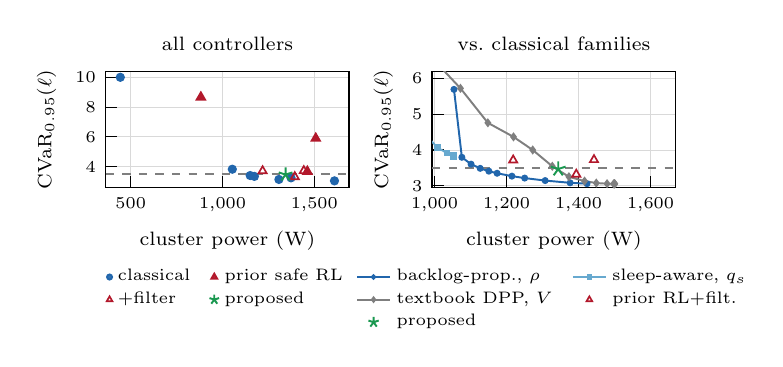
\begin{tikzpicture}
\begin{groupplot}[
  group style={group size=2 by 1, horizontal sep=30pt},
  width=88pt, height=42pt, xlabel={cluster power (W)},
  ylabel={$\mathrm{CVaR}_{0.95}(\ell)$}, legend columns=2,
  legend style={at={(0.5,-0.62)}, anchor=north, draw=none, fill=none, font=\figtick, /tikz/every even column/.append style={column sep=5pt}}]
\nextgroupplot[title={all controllers}, xmin=363.264, xmax=1690, ymin=2.6, ymax=10.4, ytick={4,6,8,10}]
\addplot[only marks, mark=*, cclassical] coordinates {(1610,3.05008) (443.264,10) (1373.28,3.25205) (1150.98,3.40799) (1173.79,3.34984) (1307.29,3.14567) (1053.43,3.83152)};
\addlegendentry{classical}
\addplot[only marks, mark=triangle*, clearned, mark size=1.7pt] coordinates {(1462.27,3.68079) (882.262,8.66282) (1508.07,5.89937)};
\addlegendentry{prior safe RL}
\addplot[only marks, mark=triangle, clearned, mark size=1.7pt, line width=0.6pt] coordinates {(1393.7,3.3204) (1218.49,3.71702) (1442.96,3.72676)};
\addlegendentry{${+}$filter}
\addplot[only marks, mark=star, cproposed, mark size=2.6pt, line width=0.7pt] coordinates {(1343.63,3.46829)};
\addlegendentry{proposed}
\addplot[cref, dashed, line width=0.6pt, forget plot] coordinates {(363.264,3.5) (1690,3.5)};
\nextgroupplot[title={vs.\ classical families}, xmin=993.432, xmax=1670, ymin=2.95, ymax=6.2, ytick={3,4,5,6}]
\addplot[cclassical, mark=*, mark size=0.9pt] coordinates {(1054.01,5.69563) (1075.92,3.7963) (1101.51,3.60356) (1126.79,3.4875) (1150.98,3.40799) (1173.79,3.34984) (1214.96,3.26937) (1250.44,3.21514) (1307.29,3.14567) (1376.74,3.08276) (1423.48,3.05822)};
\addlegendentry{backlog-prop., $\rho$}
\addplot[clight, mark=square*, mark size=0.9pt] coordinates {(830.841,7.47225) (926.866,4.95298) (1008.34,4.06503) (1034.72,3.91572) (1052.65,3.83674) (1053.43,3.83152)};
\addlegendentry{sleep-aware, $q_s$}
\addplot[cref, mark=diamond*, mark size=1.1pt] coordinates {(522.635,10) (693.99,9.77957) (1072.07,5.72492) (1148.16,4.76015) (1219.41,4.3673) (1272.76,4.00074) (1327.17,3.54543) (1373.28,3.25205) (1416.73,3.13054) (1449.38,3.07603) (1479.31,3.05882) (1497.49,3.05532) (1500.2,3.05432) (1500.53,3.05509) (1500.54,3.05432)};
\addlegendentry{textbook DPP, $V$}
\addplot[only marks, mark=triangle, clearned, mark size=1.7pt, line width=0.6pt] coordinates {(1393.7,3.3204) (1218.49,3.71702) (1442.96,3.72676)};
\addlegendentry{prior RL${+}$filt.}
\addplot[only marks, mark=star, cproposed, mark size=2.8pt, line width=0.7pt] coordinates {(1343.63,3.46829)};
\addlegendentry{proposed}
\addplot[cref, dashed, line width=0.6pt, forget plot] coordinates {(993.432,3.5) (1670,3.5)};
\end{groupplot}
\end{tikzpicture}
\end{document}
